\documentclass[12pt]{article}
\usepackage{amsthm,amssymb,amsfonts,amsmath,amstext,systeme}
\usepackage{graphicx,float}
\usepackage{tabularx}

\marginparwidth 0pt
\oddsidemargin -1.2 truecm
\evensidemargin  0pt 
\marginparsep 0pt
\topmargin -2.2truecm
\linespread{1}
\textheight 25.8 truecm
\textwidth 18.5 truecm
\newenvironment{remark}{\noindent{\bf Remark }}{\vspace{0mm}}
\newenvironment{remarks}{\noindent{\bf Remarks }}{\vspace{0mm}}
\newenvironment{question}{\noindent{\bf Question }}{\vspace{0mm}}
\newenvironment{questions}{\noindent{\bf Questions }}{\vspace{0mm}}
\newenvironment{note}{\noindent{\bf Note }}{\vspace{0mm}}
\newenvironment{summary}{\noindent{\bf Summary }}{\vspace{0mm}}
\newenvironment{back}{\noindent{\bf Background}}{\vspace{0mm}}
\newenvironment{conclude}{\noindent{\bf Conclusion}}{\vspace{0mm}}
\newenvironment{concludes}{\noindent{\bf Conclusions}}{\vspace{0mm}}
\newenvironment{dill}{\noindent{\bf Description of Dill's model}}{\vspace{0mm}}
\newenvironment{maths}{\noindent{\bf Mathematics needed}}{\vspace{0mm}}
\newenvironment{inst}{\noindent{\bf Instructions}}{\vspace{0mm}}
\newenvironment{notes}{\noindent{\bf Notes }}{\vspace{0mm}}
\newenvironment{theorem}{\noindent{\bf Theorem }}{\vspace{0mm}}
\newenvironment{example}{\noindent{\bf Example }}{\vspace{0mm}}
\newenvironment{examples}{\noindent{\bf Examples }}{\vspace{0mm}}
\newenvironment{topics}{\noindent{\bf Topics}}{\vspace{0mm}}
\newenvironment{outcomes}{\noindent{\bf Expected Learning Outcomes}}{\vspace{0mm}}
\newenvironment{lemma}{\noindent{\bf Lemma }}{\vspace{0mm}}
\newenvironment{solution}{\noindent{\it Solution}}{\vspace{2mm}}
\newcommand{\ds}{\displaystyle}
\newcommand{\un}{\underline}
\newcommand{\bs}{\boldsymbol}

\begin{document}

\baselineskip 18 pt
\begin{center}
	{\large \bf HKDSE MATH CORE 2016 Past Paper I}\\
	\vspace{2 mm}

\end{center}
\vspace{0.05cm}

\begin{enumerate}
	\item \textbf{HKDSE MATH CORE 2016 Past Paper I Q1}\\
	Simplify $\dfrac{(x^8y^7)^2}{x^5y^{-6}}$ and express your answer with positive indices. \\(3 marks)	
	
	\item \textbf{HKDSE MATH CORE 2016 Past Paper I Q2}\\
	Make $x$ the subject of the formula $Ax = (4x + B)C$. \\(3 marks)

	\item \textbf{HKDSE MATH CORE 2016 Past Paper I Q3}\\
	Simplify $\dfrac{2}{4x - 5} + \dfrac{3}{1-6x}$. \\(3 marks)

	\item \textbf{HKDSE MATH CORE 2016 Past Paper I Q4}\\
	Factorize
	\begin{enumerate}
		\item[(a)] $5m - 10n$,
		\item[(b)] $m^2 + mn - 6n^2$,
		\item[(c)] $m^2 + mn - 6n^2 - 5m + 10n$.
	\end{enumerate}
	(4 marks)

	\item \textbf{HKDSE MATH CORE 2016 Past Paper I Q5}\\
	In a recreation club, there are 180 members and the number of male members in 40\% more than the number of female members. Find the difference of the number of male members and the number of female members. \\(4 marks)
   
	\item \textbf{HKDSE MATH CORE 2016 Past Paper I Q6}\\
	Consider the compound inequality $$x + 6 < 6(x + 11) \text{ or } x \leq -5 \dots\dots\dots\dots\dots (*) .$$
	\begin{enumerate}
		\item[(a)] Solve (*).
		\item[(b)] Write down the greatest negative integer satisfying (*).
	\end{enumerate}
	(4 marks)

	\item \textbf{HKDSE MATH CORE 2016 Past Paper I Q7}\\
	In a polar coordinate system, $O$ is the pole. The polar coordinates of the points $A$ and $B$ are $(12, 75^\circ)$ and $(12, 135^\circ)$ respectively.
	\begin{enumerate}
		\item[(a)] Find $\angle APB$.
		\item[(b)] Find the perimeter of $\triangle AOB$.
		\item[(c)] Write down the number of folds of rotational symmetry of $\triangle AOB$.
	\end{enumerate}
	
	\item \textbf{HKDSE MATH CORE 2016 Past Paper I Q8}\\
	It is given that $f(x)$ is the sum of two parts, one part varies as $x$ and the other part varies as $x^2$. Suppose that $f(3) = 48$ and $f(9) = 198$.
	\begin{enumerate}
		\item[(a)] Find $f(x)$.
		\item[(b)] Solve the equation $f(x) = 90$.
	\end{enumerate}
	(5 marks)	
	
	\item \textbf{HKDSE MATH CORE 2016 Past Paper I Q9}\\
	The frequency distribution table and the cumulative frequency distribution table below show the distribution of the heights of the plants in a garden.
	\begin{table}[h]
		\centering
		\begin{minipage}{.45\textwidth}
		  \centering
		  \begin{tabular}{ | c | c | }
			\hline
			Height (m) & Frequency \\
			\hline
			$0.1 - 0.3$ & $a$ \\
			\hline
			$0.4 - 0.6$ & $4$ \\
			\hline
			$0.7 - 0.9$ & $b$ \\
			\hline
			$1.0 - 1.2$ & $c$ \\
			\hline
			$1.3 - 1.5$ & $15$ \\
			\hline
			$1.6 - 1.8$ & $3$ \\
			\hline
		  \end{tabular}
		\end{minipage}
		\hfill
		\begin{minipage}{.5\textwidth}
		  \centering
		  \begin{tabular}{ | c | c | }
			\hline
			Height less than(m)&Cumulative frequency\\
			\hline
			0.35 & 2 \\
			\hline
			0.65 & $x$ \\
			\hline
			0.95 & 13 \\
			\hline
			1.25 & $y$ \\
			\hline
			1.55 & 37 \\
			\hline
			1.85 & $z$ \\
			\hline
		  \end{tabular}
		\end{minipage}
		\label{tab:two_tables}
	\end{table}
	\begin{enumerate}
		\item[(a)] Find $x$, $y$ and $z$.
		\item[(b)] If a plant is randomly selected from the garden, find the probability that the height of the selected plant is less than 1.25 m but not less than 0.65 m.
	\end{enumerate}
	(5 marks)

	\item \textbf{HKDSE MATH CORE 2016 Past Paper I Q10}\\
	The coordinates of the points $A$ and $B$ are $(5, 7)$ and $(13, 1)$ respectively. Let $P$ be a moving point in the rectangular coordinate plane such that $P$ is equidistant from $A$ and $B$. Denote the locus of $P$ by $\Gamma$.
	\begin{enumerate}
		\item[(a)] Find the equation of $\Gamma$. \\(4 marks)
		\item[(b)] $\Gamma$ intersects the $x$-axis and the $y$-axis at $H$ and $K$ respectively. Denote the origin by $O$. Let $C$ be the circle which passes through $O$, $H$ and $K$. Someone claims that the circumference of $C$ exceeds 30. Is the claim correct? Explain your answer. \\(3 marks)
	\end{enumerate}

	\item \textbf{HKDSE MATH CORE 2016 Past Paper I Q11}\\
	An inverted right circular conical vessel contains some milk. The vessel is held vertically. The depth of milk in the vessel is 12 cm. Peter then pours $444\pi$ cm$^3$ of milk into the vessel without overflowing. He now finds that the depth of milk in the vessel is 16 cm.
	\begin{enumerate}
		\item[(a)] Express the final volume of milk in the vessel in terms of $\pi$. \\(3 marks)
		\item[(b)] Peter claims that the final area of the wet curved surface of the vessel is at least 800 cm$^2$. Do you agree? Explain your answer. \\(3 marks)
	\end{enumerate}

	\item \textbf{HKDSE MATH CORE 2016 Past Paper I Q12}\\
	The bar chart below shows the distribution of the ages of the children in a group, where $a > 11$ and $4 < b < 10$. The median of the ages in the group is 7.5.
	\begin{figure}[H]
		\centering
		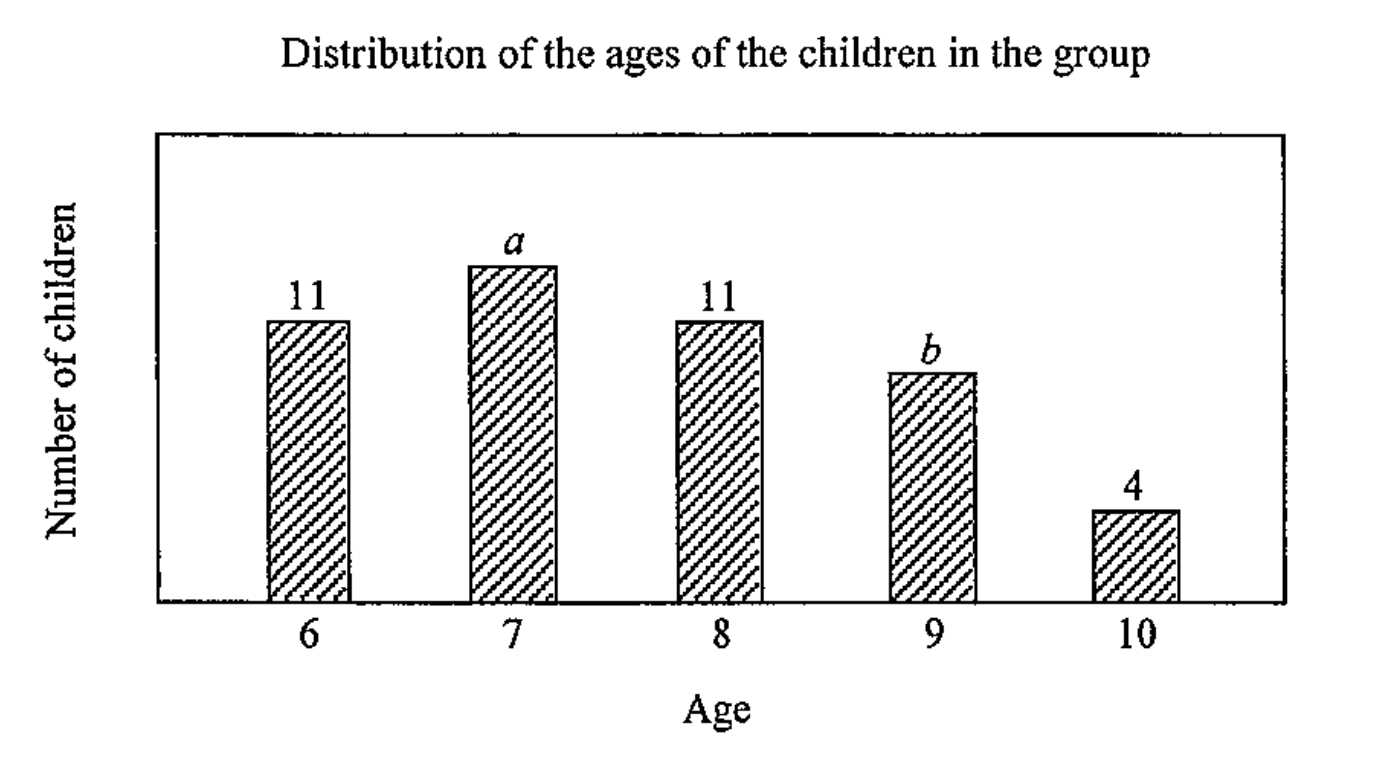
\includegraphics[width = .3\linewidth]{2016Figure1.00}
	\end{figure}
	\begin{enumerate}
		\item[(a)] Find $a$ and $b$. \\(3 marks)
		\item[(b)] Four more children now join the group. It is found that the ages of these four children are all different and the range of the ages of the children in the group remains unchanged. Find
		\begin{enumerate}
			\item[(i)] the greatest possible median of the ages of the children in the group,
			\item[(ii)] the least possible mean of the ages of the children in the group.
		\end{enumerate}
		(4 marks)
	\end{enumerate}

	\item \textbf{HKDSE MATH CORE 2016 Past Paper I Q13}\\
	In Figure 1, $ABC$ is a triangle. $D$, $E$ and $M$ are points lying on $BC$ such that $BD = CE$, $\angle ADC = \angle AEB$ and $DM = EM$.
	\begin{figure}[H]
		\centering
		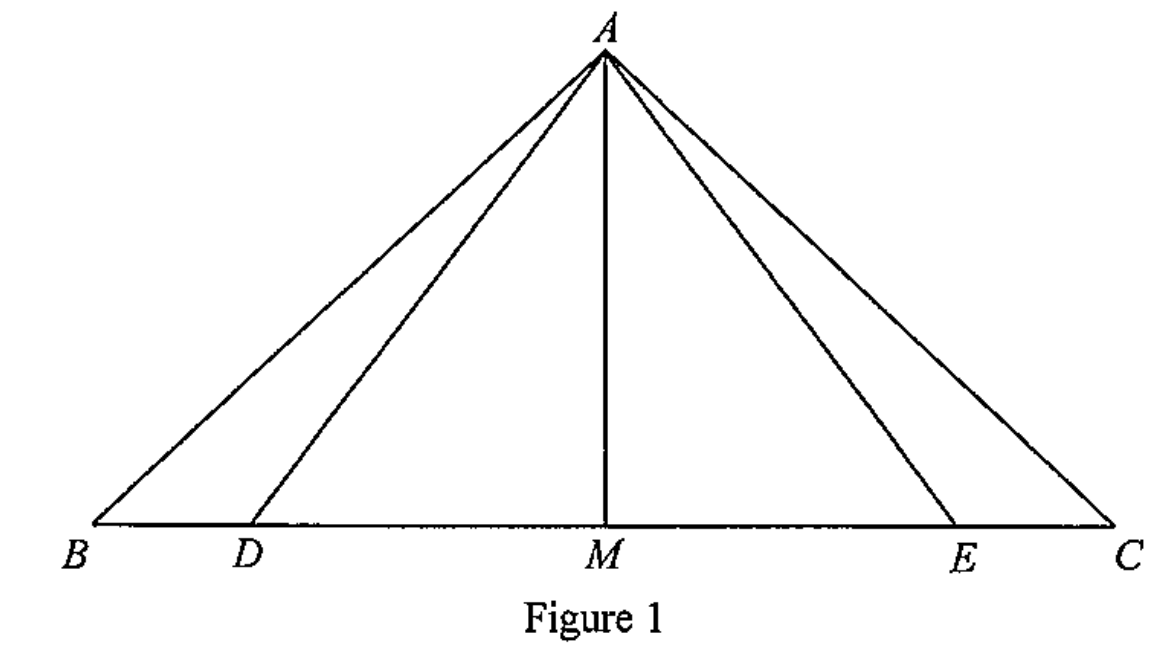
\includegraphics[width = .3\linewidth]{2016Figure1.1}
	\end{figure}
	\begin{enumerate}
		\item[(a)] Prove that $\triangle ACD \equiv \triangle ABE$. \\(2 marks)
		\item[(b)] Suppose that $AD$ = 15 cm, $BD$ = 7 cm and $DE$ = 18 cm.
		\begin{enumerate}
			\item[(i)] Find $AM$.
			\item[(ii)] Is $\triangle ABE$ a right-angled triangle? Explain your answer.
		\end{enumerate}
		(5 marks)
	\end{enumerate}

	\item \textbf{HKDSE MATH CORE 2016 Past Paper I Q14}\\
	Let $p(x) = 6x^4 + 7x^3 + ax^2 + bx + c$, where $a$, $b$ and $c$ are constants. When $p(x)$ is divided by $x + 2$ and when $p(x)$ is divided by $x - 2$, the two remainders are equal. It is given that $p(x) = (lx^2 + 5x + 8)(2x^2 + mx + n)$, where $l$, $m$ and $n$ are constants.
	\begin{enumerate}
		\item[(a)] Find $l$, $m$ and $n$. \\(5 marks)
		\item[(b)] How many real roots does the equation $p(x) = 0$ have? Explain your answer. \\(5 marks)
	\end{enumerate}

	\item \textbf{HKDSE MATH CORE 2016 Past Paper I Q15}\\
	If 4 boys and 5 girls randomly form a queue, find the probability that no boys are next to each other in the queue. \\(3 marks)

	\item \textbf{HKDSE MATH CORE 2016 Past Paper I Q16}\\
	In a test, the mean of the distribution of the scores of a class of students is 61 marks. The standard scores of Albert and Mary are $-2.6$ and 1.4 respectively. Albert gets 22 marks. A student claims that the range of the distribution is at most 59 marks. Is the claim correct? Explain your answer. \\(3 marks)

	\item \textbf{HKDSE MATH CORE 2016 Past Paper I Q17}\\
	The 1st term and the 38th term of an arithmetic sequence are 666 and 555 respectively. Find
	\begin{enumerate}
		\item[(a)] the common difference of the sequence, \\(2 marks)
		\item[(b)] the greatest value of n such that the sum of the first n terms of the sequence is positive. \\(3 marks)
	\end{enumerate}

	\item \textbf{HKDSE MATH CORE 2016 Past Paper I Q18}\\
	Let $f(x) = \dfrac{-1}{3}x^2 + 12x - 121$.
	\begin{enumerate}
		\item[(a)] Using the method of completing the square, find the coordinates of the vertex of the graph of $y = f(x)$. \\(2 marks)
		\item[(b)] The graph of $y = g(x)$ is obtained by translating the graph of $y = f(x)$ vertically. If the graph of $y = g(x)$ touches the $x$-axis, find $g(x)$. \\(2 marks)
		\item[(c)] Under a transformation, $f(x)$ is changed to $\dfrac{-1}{3}x^2 - 12x - 121$. Describe the geometric meaning of the transformation. \\(2 marks)
	\end{enumerate}

	\item \textbf{HKDSE MATH CORE 2016 Past Paper I Q19}\\
	Figure 2 shows a geometric model $ABCD$ in the form of tetrahedron. It is given that $\angle BAD = 86^\circ$, $\angle CBD = 43^\circ$, $AB$ = 10 cm, $AC$ = 6 cm, $BC$ = 8 cm and $BD = 15$ cm.
	\begin{figure}[H]
		\centering
		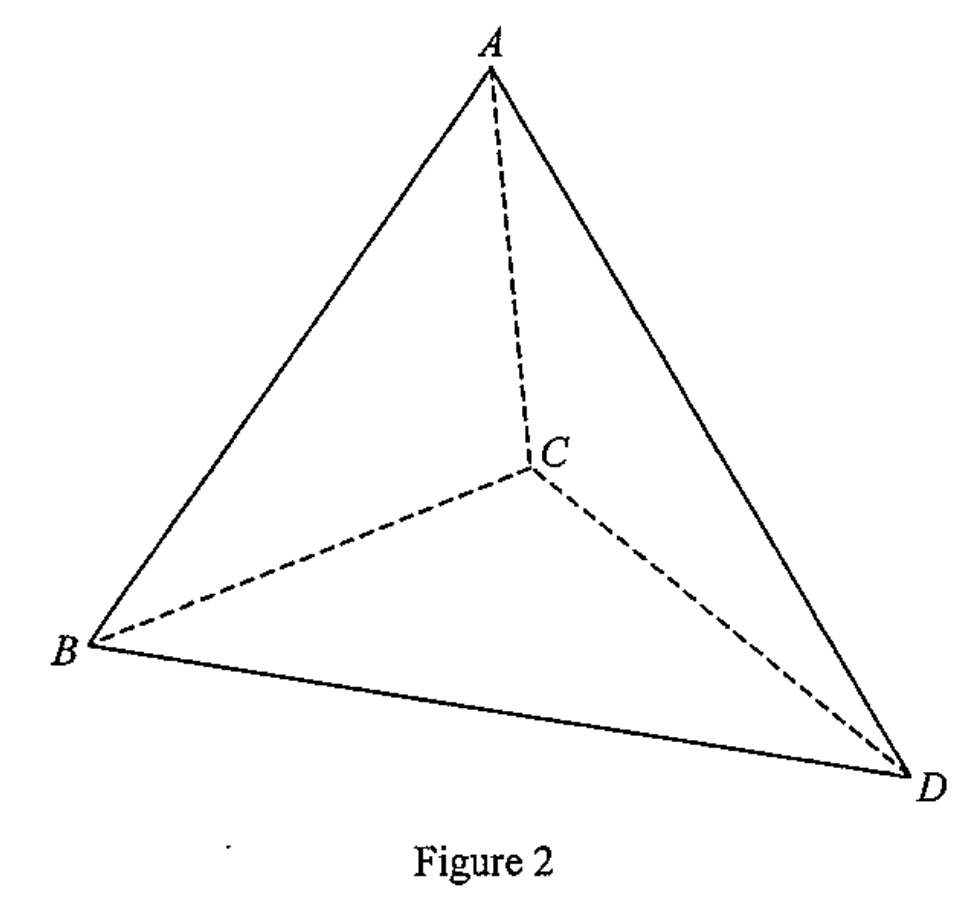
\includegraphics[width = .3\linewidth]{2016Figure1.2}
	\end{figure} 
	\begin{enumerate}
		\item[(a)] Find $\angle BAD$ and $CD$. \\(4 marks)
		\item[(b)] A craftsman claims that the angle between AB and the face $BCD$ is $\angle ABC$. Do you agree? Explain your answer. \\(2 marks)
	\end{enumerate}

	\item \textbf{HKDSE MATH CORE 2016 Past Paper I Q20}\\
	$\triangle OPQ$ is an obtuse-angled triangle. Denote the in-centre and the circumcentre of $\triangle OPQ$ by $I$ and $J$ respectively. It is given that $P$, $I$ and $J$ are collinear.
	\begin{enumerate}
		\item[(a)] Prove that $OP = PQ$. \\(3 marks)
		\item[(b)] A rectangular coordinate system is introduced so that the coordinates of O and Q are $(0, 0)$ and $(40, 30)$ respectively while the $y$-coordinate of $P$ is 19. Let $C$ be the circle which passes through $O$, $P$ and $Q$.
		\begin{enumerate}
			\item[(i)] Find the equation of $C$.
			\item[(ii)] Let $L_1$ and $L_2$ be two tangents to $C$ such that the slope of each tangent is $\dfrac{3}{4}$ and the $y$-intercept of $L_1$ is greater than that of $L_2$. $L_1$ cuts the $x$-axis and the $y$-axis at $S$ and $T$ respectively while $L_2$ cuts the $x$-axis and the $y$-axis at $U$ and $V$ respectively. Someone claims that the area of the trapezium $STUV$ exceeds 17 000. Is the claim correct? Explain your answer.
		\end{enumerate}
		(9  marks)
	\end{enumerate}
\end{enumerate}
\end{document}